\thispagestyle{empty}
%----------------------------------------------------------------------
\chapter{Modeling}
\label{modeling.chap}
%----------------------------------------------------------------------

\section{Objectives}
%----------------------------------------------------------------------

The modeling of a system starts with a good description (see Section~\ref{description.sec}). Very often, the system can is made of numerous elements (e.g. cars, particles...) or can be decomposed into small chunks (string, heated body...). In this course we want to obtain PDEs: this means that the dynamics is local. Small elements influence only their neighbors through quantities that are very important: tension and curvature for a string, density and flow for traffic... In order to obtain PDEs, it is often necessary to assume such quantities are slowly varying and that one can \emph{scale} the system. Moreover, one should keep only a very limited number of quantities and simplifying assumptions are key to that objective (neglect gravity, torsion, viscosity...). Finally, an equation (even after scaling) is always obtain as limit of another equation: it is important to explain which principles (physical or other) lead to these equations, be it a conservation equation or dynamical equations.

Now, a model is not complete with only a PDE: initial and boundary conditions must be explicit, the control parameter (or the space of choice) must be given as well as the optimization criteria. The following examples illustrate this method. 

\section{Derivation of partial differential equations}
%----------------------------------------------------------------------
This section shows how one can describe some simple systems and derive from physical principles the PDEs modeling their behavior.

\subsection{2D wave equation}
% ***********************************************************************************
% Pure LaTeX part to be inserted in a document (be careful of depencies of packages & commands
% Prepared by XXX and YYY under the supervision of Arnaud de La Fortelle
% Fall 2017
% 2D wave propagation subsection of the modeling part
% ***********************************************************************************

\subgroup{1}{Bradley Cage and Lin Yang}

\paragraph{Description}
\begin{figure}[htb]
	\centering
	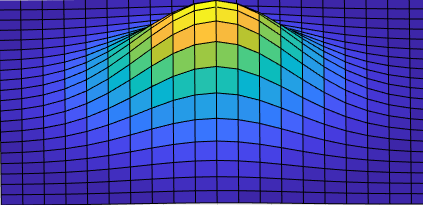
\includegraphics[width=10cm]{Figures/2D_waves_system.png}       
	\caption{The membrane system }
	\label{2D_waves_system.fig}
\end{figure}

Our system is comprised of a flexible membrane stretched to some shape, with all of its edges fixed in place. The desired goal is to understand the vertical position of the various points on the membrane over time. The membrane in this system has vertical deflections which are small compared to its overall size, and deflections happen only in the vertical direction.

This 2D system is a continuation of the 1D wave equation, and is a natural precursor to the 3D wave case. 


\paragraph{Model}
Assumptions:
\begin{itemize}
	\item Membrane has uniform planar density $\rho$
    \item The tension per unit length, $F_t$, caused by stretching the membrane is the same at all points and in all directions and does not change during the motion
    \item Vertical position is given by some function $u(x,y,t)$
\end{itemize}
\begin{figure}[htb]
	\centering
	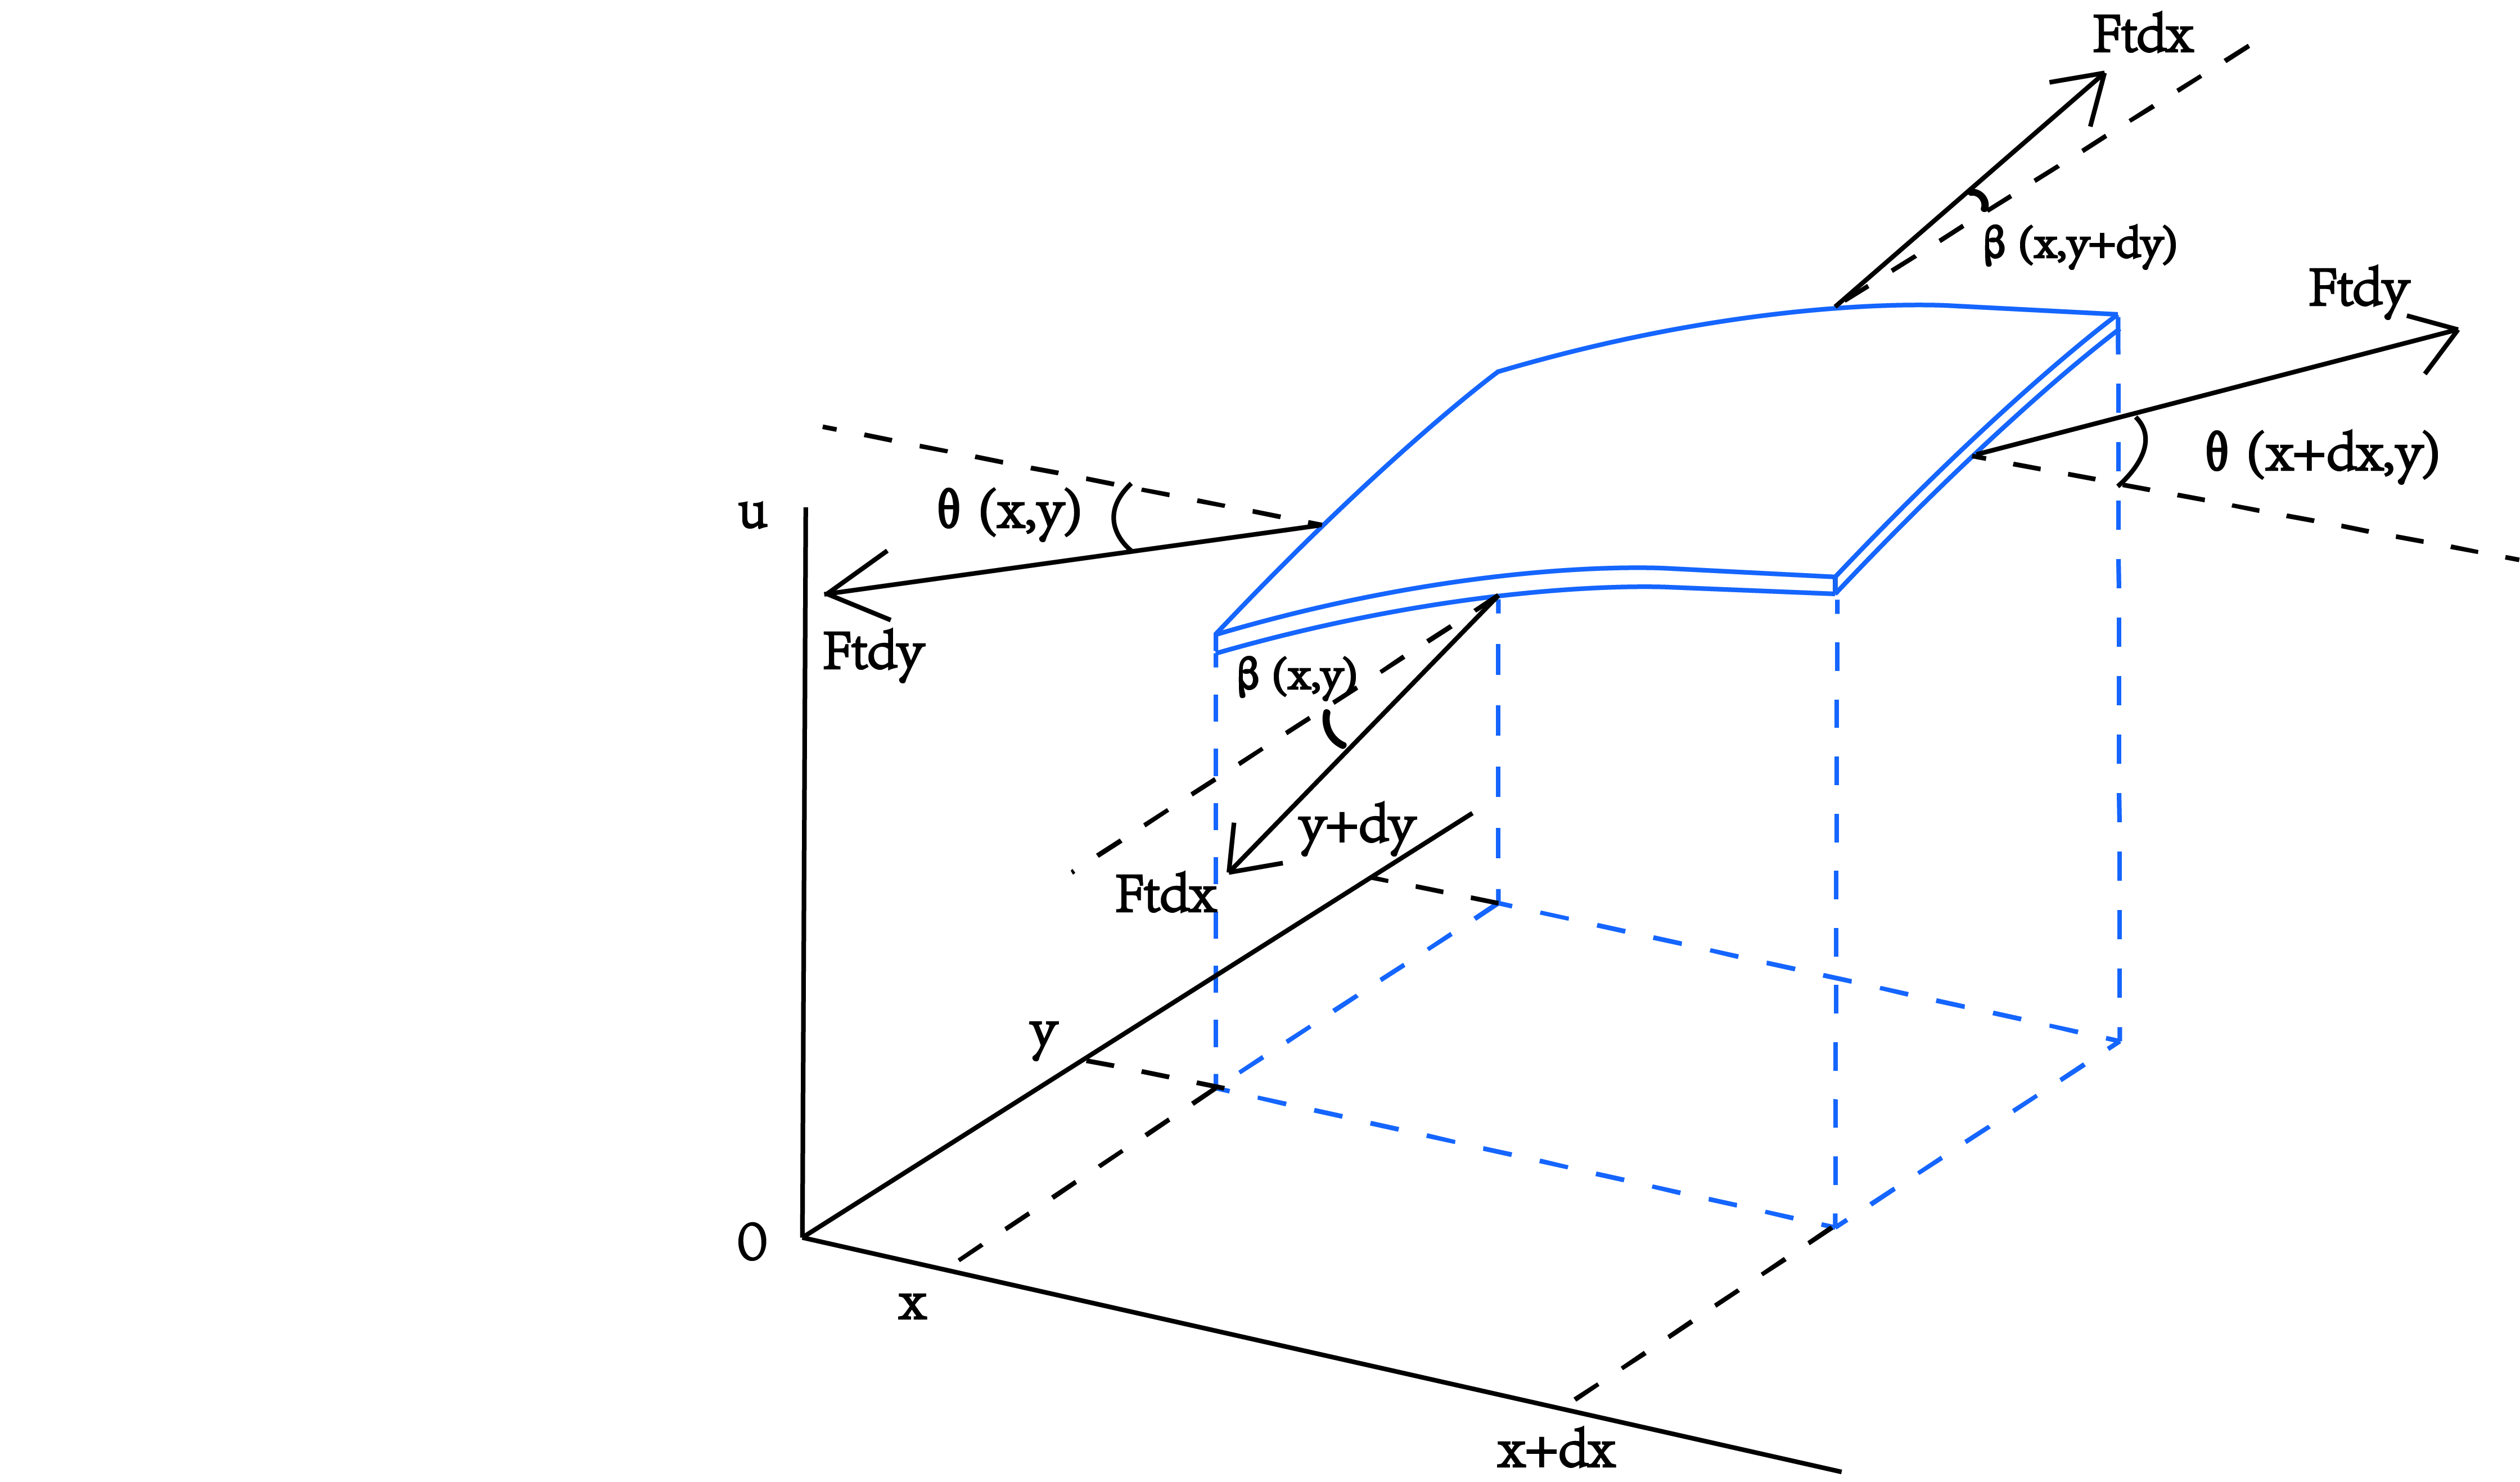
\includegraphics[width=15cm]{Figures/2D_waves_model.png}       
	\caption{The force analysis of a small section of the membrane system }
	\label{2D_waves_model.fig}
\end{figure}
We begin from basic principles.

$$\Sigma F = m\vec{a}$$

\noindent Taking some small section of the membrane $dx$ by $dy$, we can replace mass and acceleration and since we know density and that $\vec{a}$ is the second derivative of position with respect to time, thus enabling us to rewrite the equation.

\begin{equation}
\label{no_balance}
\Sigma F = \rho dxdy \frac{\partial^2u}{\partial t^2}
\end{equation}

\noindent Performing a force balance on the section of membrane in the x and y directions gives us tensions at each on each side, then resolved to their vertical components. Remember that since tension is constant per unit length, we must multiply the force acting on each side by the length of that side. Thus, the force acting on this balance lets us rewrite $\Sigma F$ (that is we only consider vertical forces, forces acting in the $x-u$ and $y-u$ planes): 

$$\Sigma F = F_x + F_y$$

$$F_x = F_tdy\Big[\sin\big( \theta (x+dx,y,t) \big) - \sin \big((\theta (x,y,t)\big)\Big]$$
$$F_y = F_tdx\Big[\sin\big( \beta (x,y+dy,t) \big) - \sin \big((\beta (x,y,t)\big)\Big]$$

\noindent We can confidently use the small angle approximation $\sin$ in the x direction

$$ \sin(\theta) \approx \tan(\theta) = \frac{\partial u}{\partial x} = u_x$$

\noindent and likewise in the y direction 

$$ \sin(\beta) \approx \tan(\beta) = \frac{\partial u}{\partial y} = u_y$$

\noindent to get our equations into the form

$$F_x = F_tdy\Big[u_x(x+dx,y,t) - u_x(x,y,t)\Big]$$
$$F_y = F_tdx\Big[u_y(x,y+dy,t) - u_y(x,y,t)\Big]$$

\noindent From there we can sum these forces and plug them back in to equation \ref{no_balance}

$$\rho dxdy \frac{\partial^2u}{\partial t^2} = F_t\bigg[dy\Big[u_x(x+dx,y,t) - u_x(x,y,t)\Big]+dx\Big[u_y(x,y+dy,t) - u_y(x,y,t)\Big] \bigg]$$

\noindent We then divide by $dx$ and $dy$ and take the limit as $dx,dy \to 0$:

$$\rho\frac{\partial^2u}{\partial t^2} = \lim_{dx,dy\to 0} F_t \bigg[ \frac{u_x(x+dx,y,t) - u_x(x,y,t)}{dx} + \frac{u_y(x,y+dy,t) - u_y(x,y,t)}{dy} \bigg]$$

\noindent We recognize that we now have derivatives in the form of difference quotients, and can take the partial derivative of each one (since $u$ is a function of multiple variables)

\begin{equation}
\rho \frac{\partial^2u}{\partial t^2} = F_t\bigg[\frac{\partial}{\partial x}u_x + \frac{\partial}{\partial y}u_y \bigg] = F_t\bigg[\frac{\partial^2 u}{\partial x^2} + \frac{\partial^2 u}{\partial y^2}\bigg]
\end{equation}

\noindent Dividing over the uniform  tension, we reach our final form.

\begin{equation}
\frac{\rho}{F_t}\frac{\partial^2u}{\partial t^2} = \frac{\partial^2 u}{\partial x^2} + \frac{\partial^2 u}{\partial y^2}
\end{equation}

\noindent We can adhere to standard conventions and write our final 2D wave equation as 


\begin{align}
a^2 \frac{\partial^2u}{\partial t^2} &= \frac{\partial^2 u}{\partial x^2} + \frac{\partial^2 u}{\partial y^2} & a &= \sqrt{\frac{\rho}{F_t}}
\label{final_eq}
\end{align}

\noindent Equation \ref{final_eq} is also commonly written using the Laplace operator:

\begin{equation}
a^2 \frac{\partial^2u}{\partial t^2} = \nabla^2 u
\end{equation}

\subsection{2D heat diffusion}
% ***********************************************************************************
% Pure LaTeX part to be inserted in a document (be careful of depencies of packages & commands)
% Prepared by XXX and YYY under the supervision of Arnaud de La Fortelle
% Fall 2017
% 2D heat diffusion subsection of the modeling part
% ***********************************************************************************

\subgroup{2}{Qingan Zhao and Ruitong Zhu}

\paragraph{Description}
The aim of this part is to describe and model a partial differential equation (PDE) that describes temperature dynamics in a two-dimensional body via heat conduction.
Basically, heat conduction is the exchange of heat from regions of higher temperatures into regions with lower temperatures, which varies in the transfer rate for different materials.
%\\\\
%COMMENT: almost never put yourself editing commands. Otherwise use LaTeX commands like \bigskip

Consider a thin flat body with a constant thickness $h$ and uniform density $\rho'$. Assume that the faces of the thin body are in perfect insulation, which means there is no heat flow travel in the out-of-plane direction of the body. Hence, heat can only flow in the direction within the plane of the body, which turns into a two-dimensional problem. Then a two-dimensional coordinate system is established such that each point of the body can be described with a coordinate $(x,y)$. Then the (2D-uniform) density of the body is $\rho = \rho' h$. Denote the temperature function of each point by $T$ so that the temperature of the body at position $(x,y)$ and time $t$ are described as $T(x,y,t)$, as shown in Figure 1. The goal is to derive $T(x,y,t)$ when there is no internal heat source.
%COMMENT: introduce your notation quickly. Best to be intuitive: T is more intuitive for temperature than u

\begin{figure}[htb]
	\centering
	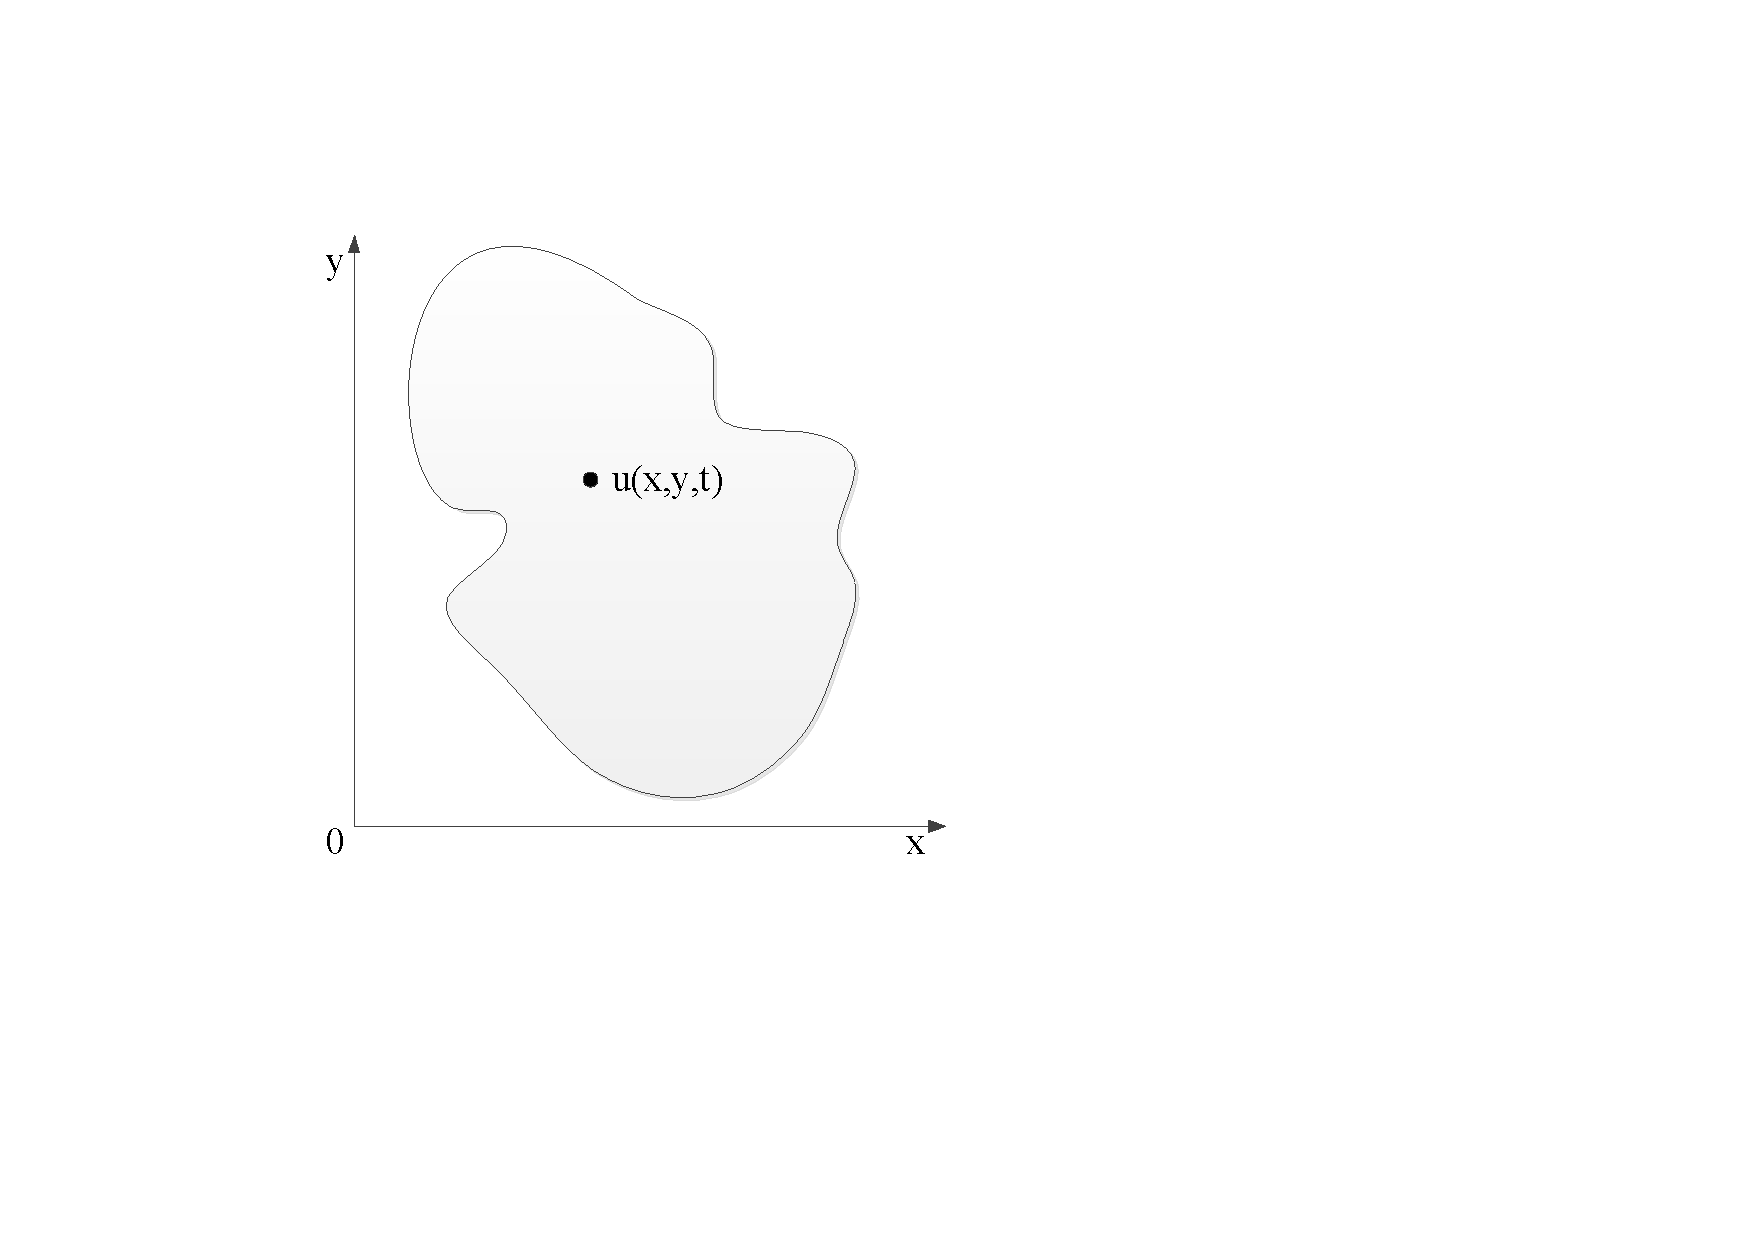
\includegraphics[width=5cm]{fig1.pdf}       
	\caption{System description in 2 dimensions}\label{heatElement.fig}
%COMMENT: do not count yourself: TODO use intensively \label and \ref
\end{figure}

\paragraph{Model}
Consider a small rectangular element of the body with vertices $(x,y)$, $(x+dx,y)$, $(x, y+dy)$, and $(x+dx, y+dy)$. The heat flows are shown in Figure 2.
\begin{figure}[htb]
	\centering
	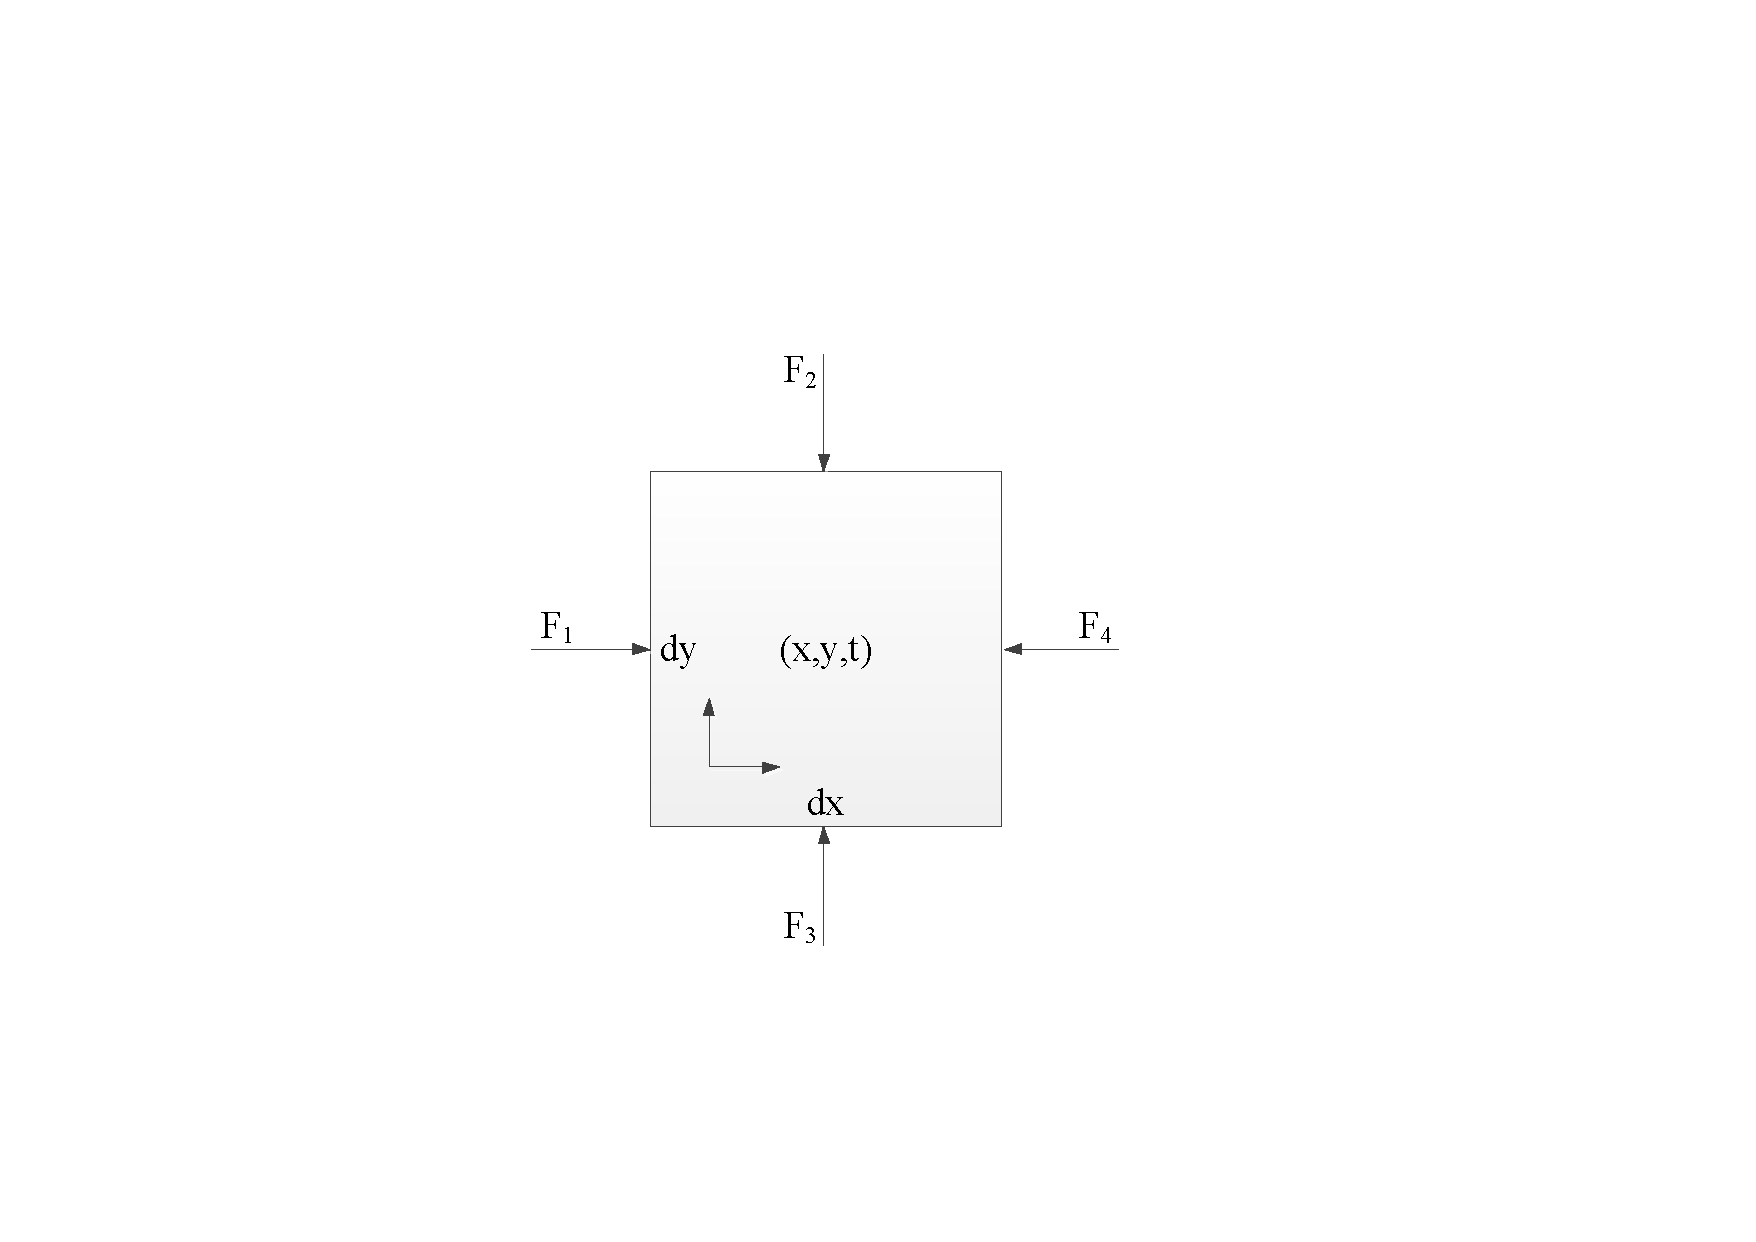
\includegraphics[width=5cm]{fig2.pdf}       
	\caption{Heat flows in a small rectangular element of the body}
\end{figure}

\noindent The heat amount $Q$ (i.e the thermal energy) of the rectangular element at time $t$ is: 
\begin{equation}
Q(x,y,t)=C m T(x,y,t)
\end{equation}
where $C$ is called \emph{heat capacity}, which is a supposed to be constant (assuming the material is uniform and temperature do not vary too much); $m = \rho A$ is the mass of the rectangular element where $A$ its surface.

The rate of thermal energy change with respect to time is therefore:
\begin{equation}\label{thermalEnergyChange.eq}
\frac{\partial Q}{\partial t} = C\rho \ud x \ud y\frac{\partial T}{\partial t}
\end{equation}
As shown in Figure~\ref{heatElement.fig}, the incoming flow is $F_1 + F_2 + F_3 + F_4$. Denote the heat flux $\vec q$ in horizontal and vertical directions by $q_x$ and $q_y$, then we have:
\begin{eqnarray} %COMMENT: the best environment for multiple equation; you can align with & as shown below TODO replace by eqnarray
F_1 &=& q_x(x,y,t)\ud y\label{flow1}\\
F_2 &=& -q_y(x,y+dy,t)dx\label{flow2}\\
F_3 &=& q_y(x,y,t)dx\label{flow3}\\
F_4 &=& -q_x(x+dx,y,t)dy\label{flow4}
\end{eqnarray}
%Sum up $F_1\sim F_4$:
%COMMENT: not very explicit, better this way:
Now, we know that according to energy conservation, the thermal energy variation of any small element (as in Equation~(\ref{thermalEnergyChange.eq})) is equal to the total incoming heat flow.  By putting the partial flows as in Equations~(\ref{flow1})-(\ref{flow4}), this conservation principle yields:
\begin{equation}\label{thermalEnergyChange.eq2}
C\rho \ud x \ud y\frac{\partial T}{\partial t} = dy [q_x(x,y,t)-q_x(x+dx,y,t)]+dxh[q_y(x,y,t)-q_y(x,y+dy,t)]
\end{equation}
%COMMENT: use \emph to emphasize
Now, another physical principle, \emph{Fourier's Law}, states that the heat flow is (negatively) proportional to the gradient of temperature:
\begin{equation}\label{FourierLaw.eq}
\vec q = -k\nabla T
\end{equation}
where $k$ is known as the thermal conductivity of the material (also considered as a constant). Then $q_x$ and $q_y$ are expressed as:
\begin{equation}
\begin{split}
q_x=-k\frac{\partial u}{\partial x}\\
q_y=-k\frac{\partial u}{\partial y}
\end{split}
\end{equation}
%TODO: replace numbers by \ref (with the appropriate \label
Hence, Equation (4) can be written as:
\begin{equation}
\frac{\partial Q}{\partial t}=kdyh[\frac{\partial u(x+dx,y,t)}{\partial x}-\frac{\partial u(x,y,t)}{\partial x}]+kdxh[\frac{\partial u(x,y+dy,t)}{\partial y}-\frac{\partial u(x,y,t)}{\partial y}]
\end{equation}
Combine Equation (2)(7):
\begin{equation}
\frac{\partial u(x,y,t)}{\partial t}=\frac{k}{c\rho}(\frac{\partial ^2 u(x,y,t)}{\partial x^2}+\frac{\partial ^2 u(x,y,t)}{\partial y^2})
\end{equation}
Denote $k/c\rho$ by $a^2$, and the two-dimensional heat equation can be drawn:
\begin{equation}
\frac{\partial u}{\partial t}=a^2\left(\frac{\partial ^2 u}{\partial x^2}+\frac{\partial ^2 u}{\partial y^2}\right)
\end{equation}
%COMMENT: look at the use of \left( and \right) to have nice parentheses



\section{Manipulation of partial differential equations}
%----------------------------------------------------------------------

\subsection{Weak formulation}
% ***********************************************************************************
% Pure LaTeX part to be inserted in a document (be careful of depencies of packages & commands)
% Prepared by XXX and YYY under the supervision of Arnaud de La Fortelle
% Fall 2017
% Derivation of the weak formulation of Dirichlet PDE; subsection of the modeling part
% ***********************************************************************************

\subgroup{3}{???}

\paragraph{Objective}

\paragraph{Demonstration}

\[u=0\\
\Delta u=\partial^2\frac{u}{x^2}+\partial^2\frac{u}{y^2}=0\\
\iint_{D}(\frac{\partial u}{\partial x}-\frac{\partial u}{\partial y})dxdy=\oint_{L}Pdx+Qdy\\
P=-\frac{\partial u}{\partial y},Q=\frac{\partial u}{\partial x}\\
\oint_{L}Pdx+Qdy=\oint_{L}(-\frac{\partial u}{\partial y}dx+\frac{\partial u}{\partial x}dy)=\oint_{L}\nabla u(-dx,dy)
\]
